%%%%%%%%%%%%%%%%%%%%
%% PSCF program
%% ~summary.tex~
%% $Rev$
%% Sept. 2009
%% Satoshi Takahama (stakahama@ucsd.edu)
%%%%%%%%%%%%%%%%%%%%

\documentclass{article}
\usepackage{graphicx}
\usepackage{nopageno}
\usepackage{fullpage}
\parindent 0pt
\begin{document}
\begin{center}
\textbf{\LARGE{Identity vs. Unique}}
\end{center}

This document compares the results of counting number of trajectory points (\verb@identity@) vs. counting the number of trajectories (\verb@unique@) for each grid cell.\\

The difference in the c.d.f. of count per cell (identity case $>$ unique case) indicates that the internal interpolation (a point each 15 minutes) results in a sufficiently dense number of points; if it were otherwise more interpolation or larger grid cells would be required.. 
\begin{center} \begin{tabular}{cc}
    Identity & Unique \\
    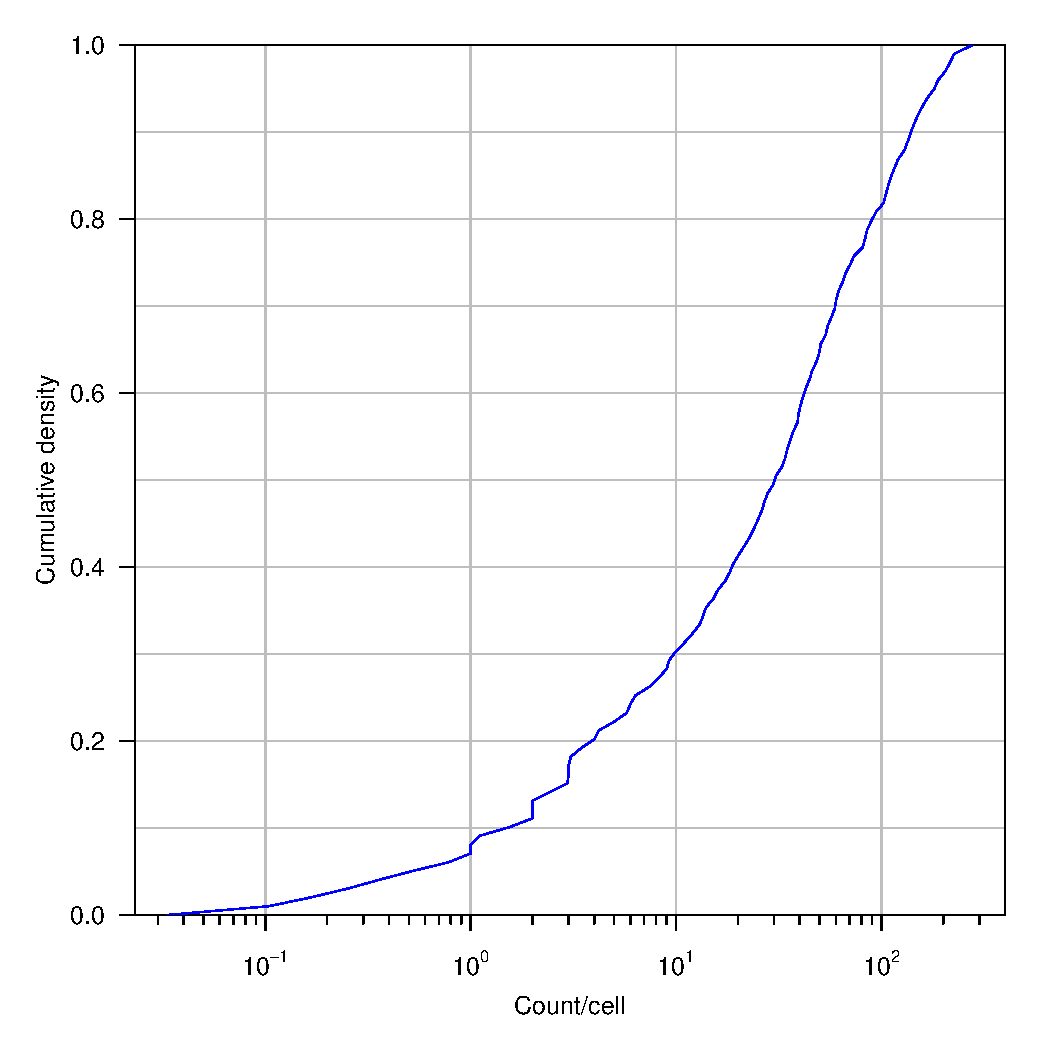
\includegraphics[width=.4\textwidth]{identitypg1.pdf} & 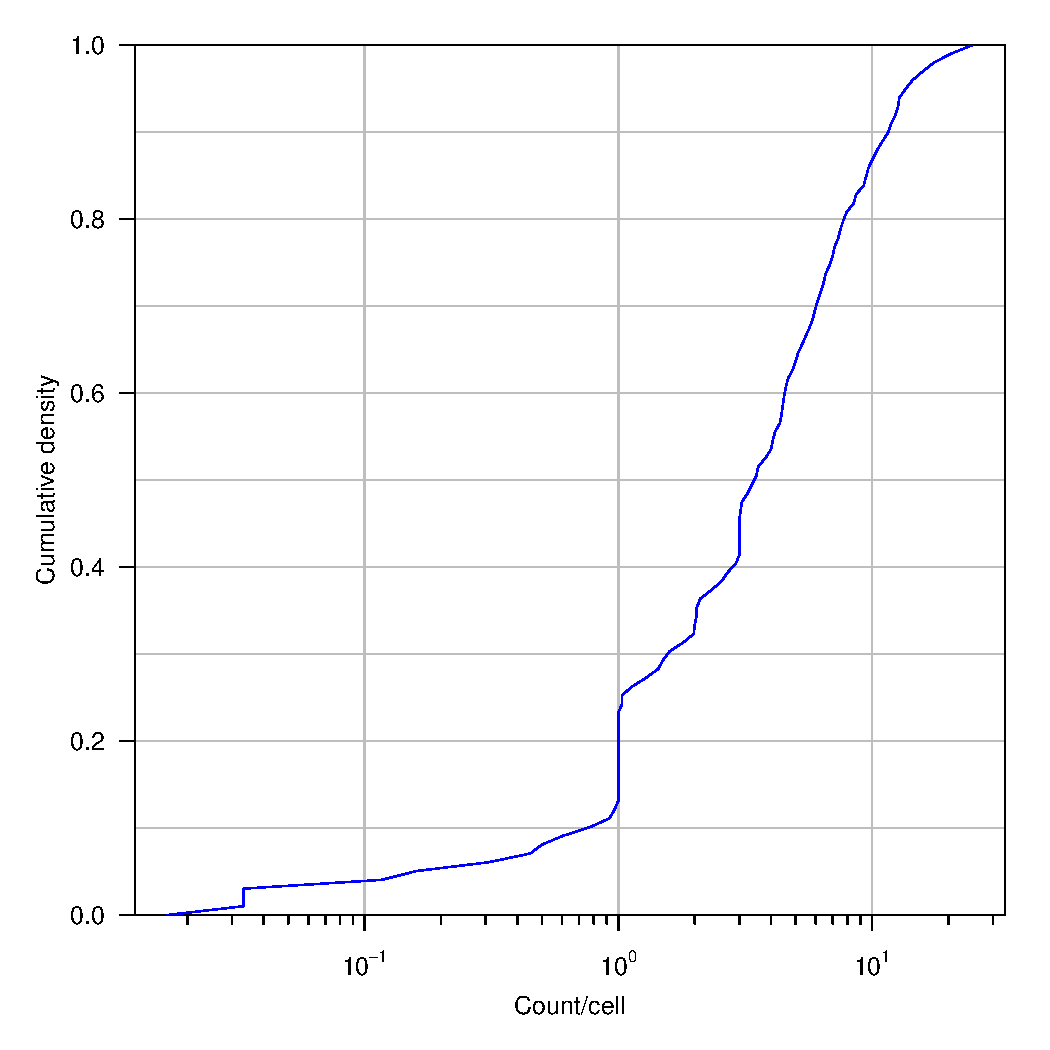
\includegraphics[width=.4\textwidth]{uniquepg1.pdf} \end{tabular} \end{center}

The PSCF results are quite similar:
\begin{center}
\begin{tabular}{cc}
Identity & Unique \\
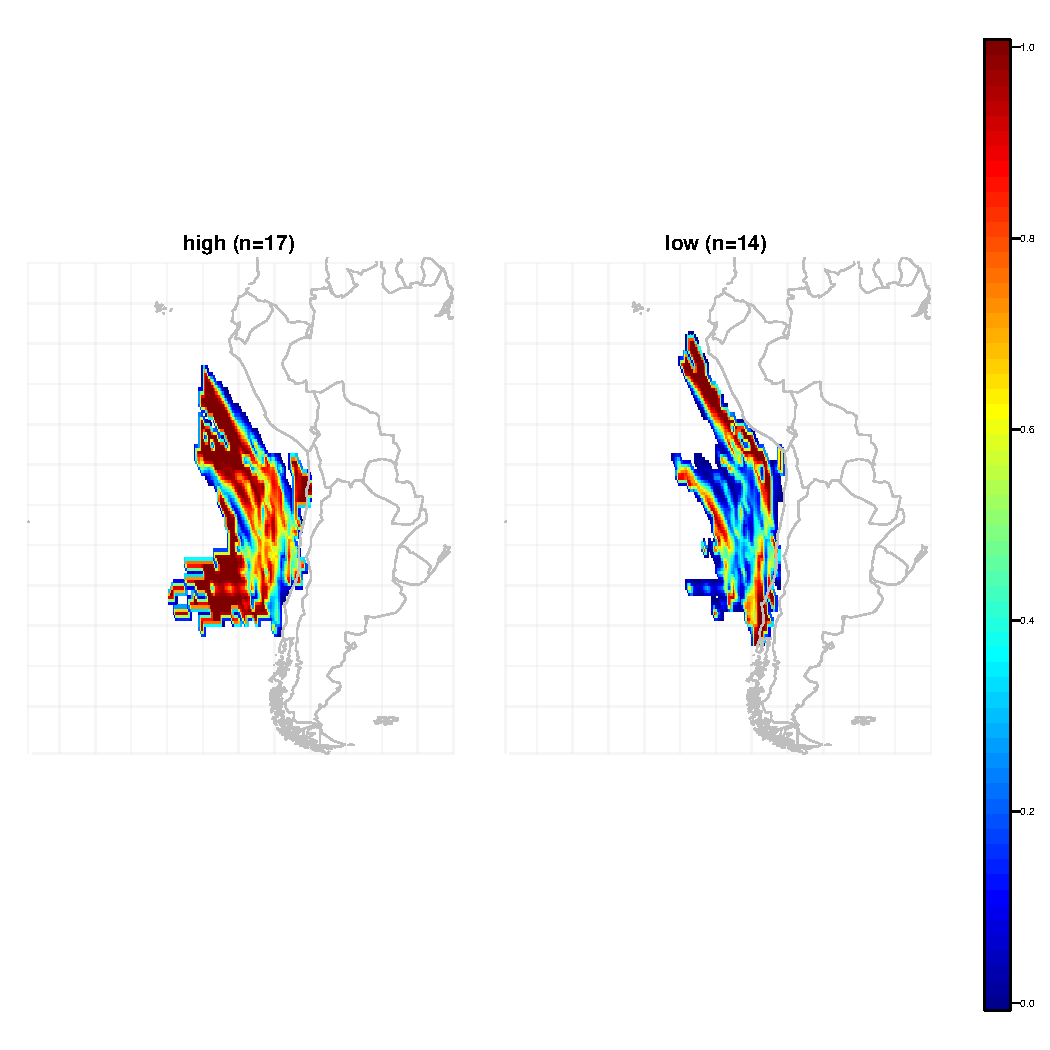
\includegraphics[width=.5\textwidth]{identitypg2.pdf} & 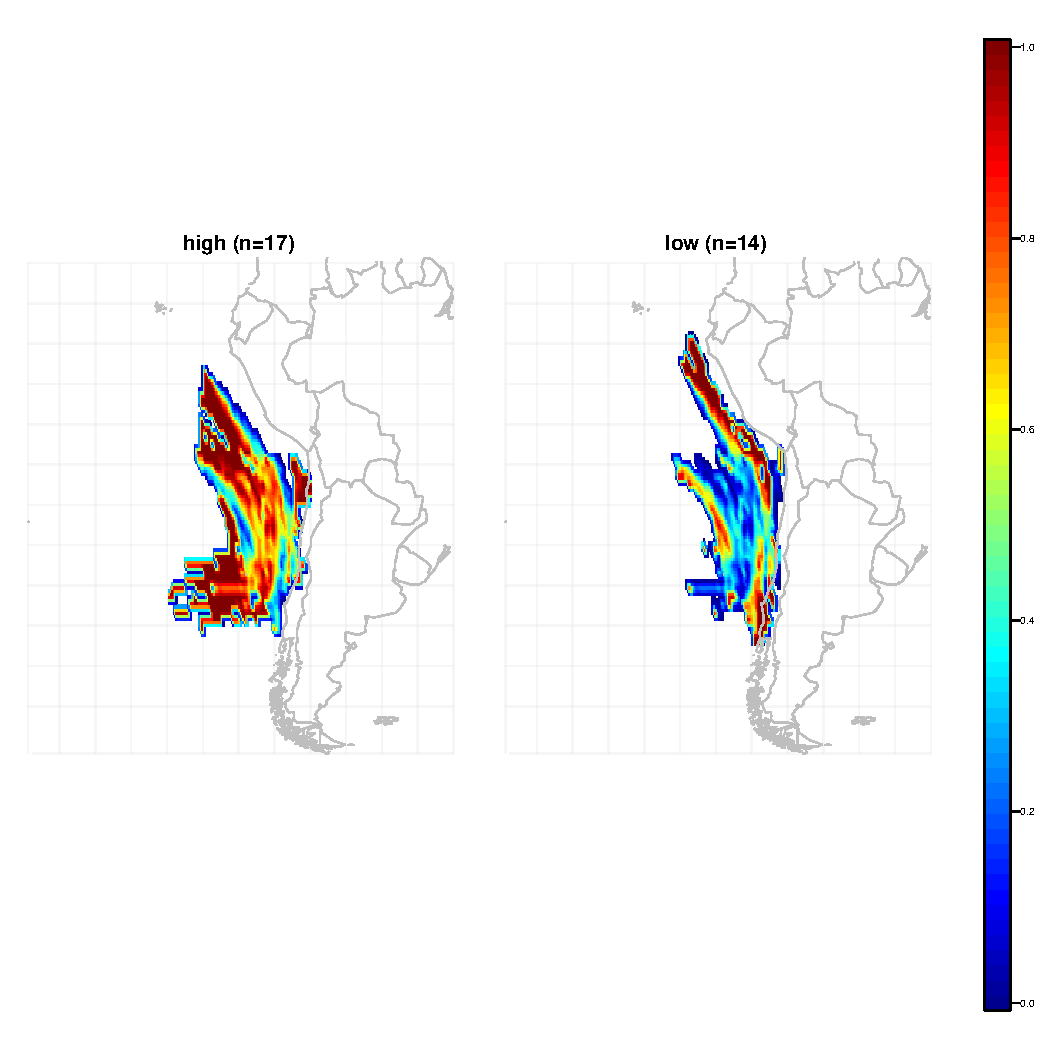
\includegraphics[width=.5\textwidth]{uniquepg2.pdf}
\end{tabular}
\end{center}

\end{document}
